%!TEX program = xelatex
%!TEX root = ../all.tex

\chapter{Nonparametric classification}

%\section*{Nonparametric Methods: Density Estimation and Classification}

\subsection*{Overview: Parametric vs.\ Nonparametric Approaches}

A large family of probabilistic classification methods can be understood as the attempt to estimate (explicitly or implicitly) posterior class probabilities and then use them to make predictions. In its simplest form, for a new input \(\mathbf{x}\) one aims to compute \(p(C_k \mid \mathbf{x})\) and then predict the most probable class. The main conceptual difference between \emph{parametric} and \emph{nonparametric} methods concerns what is assumed about the shape of the underlying distributions and, consequently, what is learned from data.

\subsubsection*{Parametric approaches}

In parametric methods, one assumes that the functional form of the relevant probability distribution is known up to a finite set of parameters, collected in a vector \(\boldsymbol{\theta}\). Learning then reduces to estimating \(\boldsymbol{\theta}\) from a training set. This assumption can be applied in two complementary ways, reflecting the two classical perspectives introduced earlier.

On the one hand, a \emph{discriminative} parametric model directly specifies the posterior distribution \(p(C_k \mid \mathbf{x}; \boldsymbol{\theta})\). Softmax regression is a standard example: the model restricts the posterior to a particular parametric family, and training adjusts \(\boldsymbol{\theta}\) so that predicted probabilities match the observed labels as closely as possible (typically by maximizing a log-likelihood or minimizing a cross-entropy loss).

On the other hand, a \emph{generative} parametric model specifies the class-conditional densities \(p(\mathbf{x}\mid C_k; \boldsymbol{\theta}_k)\) together with the class priors \(p(C_k)\). Once these quantities are available, Bayes' rule provides the posterior:
\[
p(C_k \mid \mathbf{x}) \propto p(\mathbf{x}\mid C_k)\,p(C_k).
\]
This approach is more structured because it models how data are generated within each class, and it can be used not only for classification but also for tasks such as sampling or handling missing data.

Regardless of whether the model is generative or discriminative, parameter estimation can be performed in several ways. A common approach is maximum likelihood (ML), which chooses parameters that maximize the probability of the observed data. A related approach is maximum a posteriori (MAP), which combines the likelihood with a prior distribution over parameters. More fully Bayesian approaches retain a full posterior distribution over \(\boldsymbol{\theta}\) and average predictions with respect to that posterior, thereby propagating parameter uncertainty into the predictive probabilities.

The major advantage of the parametric choice is simplicity: a compact set of parameters summarizes the training set, and learning and prediction are often computationally efficient. The main disadvantage is that performance can degrade sharply when the assumed functional form is wrong. If the model is misspecified---for instance because the true class-conditional densities are far from Gaussian while the method assumes Gaussianity---the resulting posterior probabilities can be systematically biased, leading to poor predictions.

\medskip

\subsubsection*{Nonparametric approaches}

Nonparametric methods take the opposite stance: rather than committing to a fixed parametric family, they make minimal assumptions about the shape of the distribution and attempt to estimate it directly from data. Here the complexity of the estimator grows with the dataset size: loosely speaking, the number of effective ``parameters'' is not fixed in advance, but increases as more samples become available. This flexibility allows nonparametric methods to adapt to arbitrary distributional shapes, capturing multimodality, skewness, and other deviations that would be difficult to represent with a small parametric model.

Two attractive consequences follow from this philosophy. First, nonparametric estimators can be very flexible: they may approximate complicated densities without requiring the analyst to guess a closed-form family in advance. Second, under suitable conditions and with appropriate choices of smoothing, they are \emph{consistent}: as \(n\to\infty\), they converge to the true underlying distribution.

At the same time, this flexibility comes at a price. Nonparametric methods are strongly affected by the \emph{curse of dimensionality}: in high-dimensional spaces, data become sparse and local neighborhoods contain very few points unless one uses extremely large regions. Moreover, computational cost can be substantial, because many nonparametric algorithms effectively compare a new query point to a large portion of the training set at prediction time. Finally, these methods require choosing smoothing hyperparameters (such as a bandwidth or a neighborhood size), and the quality of the results may depend crucially on this choice.

\medskip

\subsection*{Kernel Density Estimation (Parzen Windows)}

\subsubsection*{Motivation: density estimation from local counts}

The central idea behind many nonparametric density estimators is to relate probability mass to geometric volume. Consider a region \(\mathcal{R}(\mathbf{x})\) containing the point \(\mathbf{x}\). The probability mass of that region is
\begin{myequation}
P_\mathbf{x}=\int_{\mathcal{R}(\mathbf{x})} p(\mathbf{z})\,d\mathbf{z}.
\end{myequation}
Now suppose we have \(n\) i.i.d.\ samples \(\{\mathbf{x}_1,\ldots,\mathbf{x}_n\}\) drawn from the unknown density \(p\). Let \(k\) be the number of samples that fall inside \(\mathcal{R}(\mathbf{x})\). Conditional on \(P_\mathbf{x}\), the random variable \(k\) follows a binomial distribution with expected value \(E[k]=nP_\mathbf{x}\). This suggests the empirical approximation
\begin{myequation}
P_\mathbf{x}\approx \frac{k}{n}.
\end{myequation}
To turn this relationship into a density estimate, we need to connect probability mass to the value of the density at \(\mathbf{x}\). If \(\mathcal{R}(\mathbf{x})\) is sufficiently small that \(p(\mathbf{z})\) is approximately constant within the region, then
\begin{myequation}
P_\mathbf{x}\approx p(\mathbf{x})\cdot V,
\end{myequation}
where \(V = |\mathcal{R}(\mathbf{x})|\) denotes the volume of the region. Combining the last two approximations yields the fundamental relation
\begin{myequation}
p(\mathbf{x}) \approx \frac{k}{nV}.
\end{myequation}
This expression captures the basic intuition: density is large where many points fall into a small region, and small where few points occupy a large region.

There are two classical ways to exploit this identity. One may fix the region volume \(V\) (thus controlling the notion of locality) and estimate \(k\) by counting how many samples fall into the region. This gives rise to \alert{kernel density estimation}. Alternatively, one may fix \(k\) (thus guaranteeing a fixed amount of data support) and then let the region grow until it contains exactly \(k\) neighbors. This yields the \alert{\(k\)-nearest neighbors} approach. These two methods share the same starting point but implement the locality assumption in different ways.

\medskip

\subsubsection*{Kernel density estimation with fixed volume}

In kernel density estimation (also known as Parzen window estimation), we center around \(\mathbf{x}\) a region of fixed volume and count how many training points fall inside it. In \(d\) dimensions, a simple choice is a hypercube of side length \(h\), whose volume is \(V=h^d\). The counting mechanism can be expressed through a kernel function \(k(\mathbf{z})\) that indicates whether a point lies in the unit hypercube:
\begin{myequation}
k(\mathbf{z})=
\begin{cases}
1 & \text{if } |z_i|\leq \frac{1}{2}\ \text{for all } i=1,\ldots,d,\\
0 & \text{otherwise}.
\end{cases}
\end{myequation}
The rescaled expression \(k\!\left(\frac{\mathbf{x}-\mathbf{x}_i}{h}\right)\) equals \(1\) if and only if \(\mathbf{x}_i\) falls within the hypercube of side length \(h\) centered at \(\mathbf{x}\). Therefore, the number of points inside the region is
\[
k = \sum_{i=1}^n k\!\left(\frac{\mathbf{x}-\mathbf{x}_i}{h}\right),
\]
and substituting into \(\frac{k}{nV}\) yields the Parzen estimate
\begin{myequation}
p_n(\mathbf{x})=\frac{1}{nh^d}\sum_{i=1}^{n} k\left(\frac{\mathbf{x}-\mathbf{x}_i}{h}\right).
\end{myequation}

This estimator has two fundamental properties that make it a meaningful candidate for a density estimate. First, it is nonnegative because it is an average of nonnegative kernel evaluations. Second, with suitable conditions on the kernel, it integrates to \(1\), thereby defining a valid probability density. Conceptually, the estimate can also be viewed as a sum of ``bumps'' centered at the data points: each observation contributes a local mass of size \(1/n\), spread over a region whose width is controlled by \(h\).

A crucial role is played by the bandwidth parameter \(h\). Choosing \(h\) is not merely a technical detail: it expresses how local the estimator should be. If \(h\) is large, each region contains many points and the estimate becomes smooth; this tends to reduce variance but can introduce bias by oversmoothing important structure. If \(h\) is small, the estimator becomes sensitive to fine detail and can capture sharp features, but the estimate may become noisy, with high variance, because each region contains only a few points.

\medskip

\subsubsection*{Histogram illustration of the bandwidth effect}

The bandwidth effect can be visualized in the simplest setting of one-dimensional histograms. The following figure shows how varying \(h\) changes the smoothness of the resulting density estimate, ranging from a very rough, highly variable estimate (small \(h\)) to an overly smooth one (large \(h\)).

\begin{figure}[h]
\begin{tikzpicture}[fill=blue!20, every path/.style={draw}, lbl/.style={circle}]

\draw [->,>=stealth'](-5,8) --(5,8);
\draw [->,>=stealth'](-5,8) --(-5,9);
\draw [-,>=stealth'](-4.5,7.9) --(-4.5,8.1);
\draw [-,>=stealth'](-4,7.9) --(-4,8.1);
\draw [-,>=stealth'](-3.5,7.9) --(-3.5,8.1);
\draw [-,>=stealth'](-3,7.9) --(-3,8.1);
\draw [-,>=stealth'](-2.5,7.9) --(-2.5,8.1);
\draw [-,>=stealth'](-2,7.9) --(-2,8.1);
\draw [-,>=stealth'](-1.5,7.9) --(-1.5,8.1);
\draw [-,>=stealth'](-1,7.9) --(-1,8.1);
\draw [-,>=stealth'](-.5,7.9) --(-.5,8.1);
\draw [-,>=stealth'](0,7.9) --(0,8.1);
\draw [-,>=stealth'](4.5,7.9) --(4.5,8.1);
\draw [-,>=stealth'](4,7.9) --(4,8.1);
\draw [-,>=stealth'](3.5,7.9) --(3.5,8.1);
\draw [-,>=stealth'](3,7.9) --(3,8.1);
\draw [-,>=stealth'](2.5,7.9) --(2.5,8.1);
\draw [-,>=stealth'](2,7.9) --(2,8.1);
\draw [-,>=stealth'](1.5,7.9) --(1.5,8.1);
\draw [-,>=stealth'](1,7.9) --(1,8.1);
\draw [-,>=stealth'](.5,7.9) --(.5,8.1);

\fill (-3.5,8.1) circle(.05);
\fill (-3,8.1) circle(.05);
\fill (-2.5,8.2) circle(.05);
\fill (-2.5,8.3) circle(.05);
\fill (-2.5,8.1) circle(.05);
\fill (-2,8.1) circle(.05);
\fill (-1.5,8.1) circle(.05);
\fill (-1.5,8.2) circle(.05);
\fill (-1,8.1) circle(.05);
\fill (-1,8.2) circle(.05);
\fill (-1,8.3) circle(.05);
\fill (0,8.1) circle(.05);
\fill (0,8.2) circle(.05);
\fill (.5,8.1) circle(.05);
\fill (.5,8.2) circle(.05);
\fill (.5,8.3) circle(.05);
\fill (.5,8.4) circle(.05);
\fill (1,8.1) circle(.05);
\fill (1,8.2) circle(.05);
\fill (1.5,8.1) circle(.05);
\fill (1.5,8.2) circle(.05);
\fill (2,8.1) circle(.05);
\fill (2,8.2) circle(.05);
\fill (2,8.3) circle(.05);
\fill (2.5,8.1) circle(.05);
\fill (3.5,8.1) circle(.05);
\fill (3.5,8.2) circle(.05);
\fill (4,8.1) circle(.05);
\fill (4,8.2) circle(.05);
\fill (4.5,8.1) circle(.05);

\draw [->,>=stealth'](-5,6) --(5,6);
\draw [->,>=stealth'](-5,6) --(-5,7);
\draw [-,>=stealth'](-4.5,5.9) --(-4.5,6.1);
\draw [-,>=stealth'](-4,5.9) --(-4,6.1);
\draw [-,>=stealth'](-3.5,5.9) --(-3.5,6.1);
\draw [-,>=stealth'](-3,5.9) --(-3,6.1);
\draw [-,>=stealth'](-2.5,5.9) --(-2.5,6.1);
\draw [-,>=stealth'](-2,5.9) --(-2,6.1);
\draw [-,>=stealth'](-1.5,5.9) --(-1.5,6.1);
\draw [-,>=stealth'](-1,5.9) --(-1,6.1);
\draw [-,>=stealth'](-.5,5.9) --(-.5,6.1);
\draw [-,>=stealth'](0,5.9) --(0,6.1);
\draw [-,>=stealth'](4.5,5.9) --(4.5,6.1);
\draw [-,>=stealth'](4,5.9) --(4,6.1);
\draw [-,>=stealth'](3.5,5.9) --(3.5,6.1);
\draw [-,>=stealth'](3,5.9) --(3,6.1);
\draw [-,>=stealth'](2.5,5.9) --(2.5,6.1);
\draw [-,>=stealth'](2,5.9) --(2,6.1);
\draw [-,>=stealth'](1.5,5.9) --(1.5,6.1);
\draw [-,>=stealth'](1,5.9) --(1,6.1);
\draw [-,>=stealth'](.5,5.9) --(.5,6.1);

\draw [red, -,>=stealth'](-5,6) --(-4.5,6);
\draw [red, -,>=stealth'](-4.5,6) --(-4.5,6.1);
\draw [red, -,>=stealth'](-4.5,6.1) --(-4,6.1);
\draw [red, -,>=stealth'](-4,6.1) --(-4,6.2);
\draw [red, -,>=stealth'](-4,6.2) --(-3.5,6.2);
\draw [red, -,>=stealth'](-3.5,6.2) --(-3.5,6.5);
\draw [red, -,>=stealth'](-3.5,6.5) --(-3,6.5);
\draw [red, -,>=stealth'](-3,6.5) --(-3,6.6);
\draw [red, -,>=stealth'](-3,6.6) --(-2.5,6.6);
\draw [red, -,>=stealth'](-2.5,6.6) --(-2.5,6.7);
\draw [red, -,>=stealth'](-2.5,6.7) --(-2,6.7);
\draw [red, -,>=stealth'](-2,6.7) --(-2,6.9);
\draw [red, -,>=stealth'](-2,6.9) --(-1.5,6.9);
\draw [red, -,>=stealth'](-1.5,6.9) --(-1.5,6.6);
\draw [red, -,>=stealth'](-1.5,6.6) --(-1,6.6);
\draw [red, -,>=stealth'](-1,6.6) --(-1,6.7);
\draw [red, -,>=stealth'](-1,6.7) --(-.5,6.7);
\draw [red, -,>=stealth'](-.5,6.7) --(-.5,6.9);
\draw [red, -,>=stealth'](-.5,6.9) --(0,6.9);
\draw [red, -,>=stealth'](0,6.9) --(0,6.8);
\draw [red, -,>=stealth'](0,6.8) --(.5,6.8);
\draw [red, -,>=stealth'](.5,6.8) --(.5,7);
\draw [red, -,>=stealth'](.5,7) --(1,7);
\draw [red, -,>=stealth'](1,7) --(1,7.1);
\draw [red, -,>=stealth'](1,7.1) --(1.5,7.1);
\draw [red, -,>=stealth'](1.5,7.1) --(1.5,6.8);
\draw [red, -,>=stealth'](1.5,6.8) --(2,6.8);
\draw [red, -,>=stealth'](2,6.8) --(2,6.6);
\draw [red, -,>=stealth'](2,6.6) --(2.5,6.6);
\draw [red, -,>=stealth'](2.5,6.6) --(3,6.6);
\draw [red, -,>=stealth'](3,6.6) --(3,6.5);
\draw [red, -,>=stealth'](3,6.5) --(3.5,6.5);
\draw [red, -,>=stealth'](3.5,6.5) --(4.5,6.5);
\draw [red, -,>=stealth'](4.5,6.5) --(4.5,6.3);
\draw [red, -,>=stealth'](4.5,6.3) --(5,6.3);

\draw [->,>=stealth'](-5,4) --(5,4);
\draw [->,>=stealth'](-5,4) --(-5,5);
\draw [-,>=stealth'](-4.5,3.9) --(-4.5,4.1);
\draw [-,>=stealth'](-4,3.9) --(-4,4.1);
\draw [-,>=stealth'](-3.5,3.9) --(-3.5,4.1);
\draw [-,>=stealth'](-3,3.9) --(-3,4.1);
\draw [-,>=stealth'](-2.5,3.9) --(-2.5,4.1);
\draw [-,>=stealth'](-2,3.9) --(-2,4.1);
\draw [-,>=stealth'](-1.5,3.9) --(-1.5,4.1);
\draw [-,>=stealth'](-1,3.9) --(-1,4.1);
\draw [-,>=stealth'](-.5,3.9) --(-.5,4.1);
\draw [-,>=stealth'](0,3.9) --(0,4.1);
\draw [-,>=stealth'](4.5,3.9) --(4.5,4.1);
\draw [-,>=stealth'](4,3.9) --(4,4.1);
\draw [-,>=stealth'](3.5,3.9) --(3.5,4.1);
\draw [-,>=stealth'](3,3.9) --(3,4.1);
\draw [-,>=stealth'](2.5,3.9) --(2.5,4.1);
\draw [-,>=stealth'](2,3.9) --(2,4.1);
\draw [-,>=stealth'](1.5,3.9) --(1.5,4.1);
\draw [-,>=stealth'](1,3.9) --(1,4.1);
\draw [-,>=stealth'](.5,3.9) --(.5,4.1);

\draw [red, -,>=stealth'](-5,4) --(-4,4);
\draw [red, -,>=stealth'](-4,4) --(-4,4.2);
\draw [red, -,>=stealth'](-4,4.2) --(-3.5,4.2);
\draw [red, -,>=stealth'](-3.5,4.2) --(-3.5,4.4);
\draw [red, -,>=stealth'](-3.5,4.4) --(-3,4.4);
\draw [red, -,>=stealth'](-3,4.4) --(-3,4.8);
\draw [red, -,>=stealth'](-3,4.8) --(-2,4.8);
\draw [red, -,>=stealth'](-2,4.8) --(-2,4.6);
\draw [red, -,>=stealth'](-2,4.6) --(-1.5,4.6);
\draw [red, -,>=stealth'](-1.5,4.6) --(-1.5,5);
\draw [red, -,>=stealth'](-1.5,5) --(-1,5);
\draw [red, -,>=stealth'](-1,5) --(-1,4.6);
\draw [red, -,>=stealth'](-1,4.6) --(-.5,4.6);
\draw [red, -,>=stealth'](-.5,4.6) --(-.5,4.4);
\draw [red, -,>=stealth'](-.5,4.4) --(0,4.4);
\draw [red, -,>=stealth'](0,4.4) --(0,5.2);
\draw [red, -,>=stealth'](0,5.2) --(1,5.2);
\draw [red, -,>=stealth'](1,5.2) --(1,4.8);
\draw [red, -,>=stealth'](1,4.8) --(1.5,4.8);
\draw [red, -,>=stealth'](1.5,4.8) --(1.5,5);
\draw [red, -,>=stealth'](1.5,5) --(2,5);
\draw [red, -,>=stealth'](2,5) --(2,4.8);
\draw [red, -,>=stealth'](2,4.8) --(2.5,4.8);
\draw [red, -,>=stealth'](2.5,4.8) --(2.5,4.2);
\draw [red, -,>=stealth'](2.5,4.2) --(3,4.2);
\draw [red, -,>=stealth'](3,4.2) --(3,4.4);
\draw [red, -,>=stealth'](3,4.4) --(3.5,4.4);
\draw [red, -,>=stealth'](3.5,4.4) --(3.5,4.8);
\draw [red, -,>=stealth'](3.5,4.8) --(4,4.8);
\draw [red, -,>=stealth'](4,4.8) --(4,4.6);
\draw [red, -,>=stealth'](4,4.6) --(4.5,4.6);
\draw [red, -,>=stealth'](4.5,4.6) --(4.5,4.2);
\draw [red, -,>=stealth'](4.5,4.2) --(5,4.2);

\draw [->,>=stealth'](-5,2) --(5,2);
\draw [->,>=stealth'](-5,2) --(-5,3);
\draw [-,>=stealth'](-4.5,1.9) --(-4.5,2.1);
\draw [-,>=stealth'](-4,1.9) --(-4,2.1);
\draw [-,>=stealth'](-3.5,1.9) --(-3.5,2.1);
\draw [-,>=stealth'](-3,1.9) --(-3,2.1);
\draw [-,>=stealth'](-2.5,1.9) --(-2.5,2.1);
\draw [-,>=stealth'](-2,1.9) --(-2,2.1);
\draw [-,>=stealth'](-1.5,1.9) --(-1.5,2.1);
\draw [-,>=stealth'](-1,1.9) --(-1,2.1);
\draw [-,>=stealth'](-.5,1.9) --(-.5,2.1);
\draw [-,>=stealth'](0,1.9) --(0,2.1);
\draw [-,>=stealth'](4.5,1.9) --(4.5,2.1);
\draw [-,>=stealth'](4,1.9) --(4,2.1);
\draw [-,>=stealth'](3.5,1.9) --(3.5,2.1);
\draw [-,>=stealth'](3,1.9) --(3,2.1);
\draw [-,>=stealth'](2.5,1.9) --(2.5,2.1);
\draw [-,>=stealth'](2,1.9) --(2,2.1);
\draw [-,>=stealth'](1.5,1.9) --(1.5,2.1);
\draw [-,>=stealth'](1,1.9) --(1,2.1);
\draw [-,>=stealth'](.5,1.9) --(.5,2.1);

% (The rest of the histogram illustration is unchanged; omitted here for brevity in comments.)
% NOTE: Keep the remaining red bars and labels exactly as in the original figure code.
\draw(-6,2.5) node {\footnotesize $h=\varepsilon$};
\draw(-6,4.5) node {\footnotesize $h=1$};
\draw(-6,6.5) node {\footnotesize $h=2$};
\end{tikzpicture}
\end{figure}

The figure highlights a key principle that will reappear throughout nonparametric learning. If \(h\) is too large, the estimate is overly smooth and may wash out structure (high bias). If \(h\) is too small, the estimate follows the random fluctuations of the sample (high variance). Selecting \(h\) amounts to choosing a compromise between these two sources of error.

\medskip

\subsubsection*{Smooth kernels and the Parzen window viewpoint}

The hypercube kernel above is essentially the kernel underlying histograms: it is simple but introduces discontinuities, and it weights all points inside the region equally, regardless of their distance from \(\mathbf{x}\). In many applications, it is preferable to use \alert{smooth kernels} that give higher weight to samples close to \(\mathbf{x}\) and lower weight to samples further away, thereby producing continuous density estimates and often better practical behavior.

A convenient way to formalize this is to introduce a family of kernels \(\kappa_h(\mathbf{u})\) parameterized by a bandwidth \(h>0\). In typical constructions one starts from a base kernel \(\kappa(\mathbf{u})\) and defines a scaled version so that its mass is preserved as \(h\) changes. Independently of the specific functional form, a valid kernel used for density estimation is commonly required to integrate to one and to be centered:
\begin{myalign}
\int \kappa_h(\mathbf{u})\, d\mathbf{u} &= 1,\\
\mathbb{E}[\mathbf{u}] = \int \mathbf{u}\,\kappa_h(\mathbf{u})\, d\mathbf{u} &= \mathbf{0},\\
\mathbb{E}[\mathbf{u}^2] = \int \mathbf{u}^2\,\kappa_h(\mathbf{u})\, d\mathbf{u} &> 0.
\end{myalign}
The first condition ensures that the kernel contributes unit mass, so that averaging over kernels yields a normalized density estimate. The second and third conditions encode symmetry and non-degeneracy: on average the kernel does not shift mass away from the center, and it has positive spread.

With a smooth kernel, the Parzen window estimate takes the compact and intuitive form
\begin{myequation}
p(\mathbf{x}) = \frac{1}{n}\sum_{i=1}^{n}\kappa_h(\mathbf{x}-\mathbf{x}_i),
\end{myequation}
which can again be interpreted as placing around each sample \(\mathbf{x}_i\) a small ``bump'' of mass \(1/n\) and summing them to obtain an overall density estimate.

Two kernels are often used as canonical examples. The \emph{Gaussian kernel} produces an infinitely smooth estimate with infinite support:
\[
\kappa_h(\mathbf{u})=\frac{1}{(\sqrt{2\pi}h)^d}\exp\!\left(-\frac{\|\mathbf{u}\|^2}{2h^2}\right).
\]
The \emph{Epanechnikov kernel} has compact support and can be computationally efficient:
\[
\kappa_h(\mathbf{u})=\frac{3}{4h}\left(1-\frac{\mathbf{u}^2}{h^2}\right)\quad \text{for } |\mathbf{u}|\le h,
\qquad
\kappa_h(\mathbf{u})=0 \ \text{otherwise}.
\]
Although these kernels differ, the general role of \(h\) remains the same: it controls the locality and therefore the bias--variance trade-off of the estimate.

\medskip

\subsubsection*{Kernel shape comparison}

Figure~\ref{f:kernels} illustrates the qualitative differences between a discontinuous histogram kernel and two smooth alternatives (Gaussian and Epanechnikov). The key point is not that one kernel is universally best, but that the kernel choice affects smoothness and computational properties, while the bandwidth \(h\) largely governs the effective resolution of the estimate.

\begin{figure}[h!]
\centering
\begin{subfigure}{0.32\textwidth}
\centering
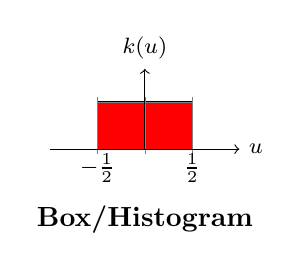
\begin{tikzpicture}[scale=.6,domain=-1:1]
\fill[color=red, samples=50] plot (-1,0)--(-1,1)--(1,1)--(1,0)--cycle;
\draw[color=black, samples=50] (-1,0)--(-1,1)--(1,1)--(1,0);
  \draw[very thin,color=gray] (-1,-0.1) grid (1,1.1);
  \draw[->] (-2,0) -- (2,0) node[right] {\footnotesize $u$};
  \draw[->] (0,0) -- (0,1.7) node[above] {\footnotesize $k(u)$};
  \draw(1,-0.4) node {\footnotesize $\frac{1}{2}$};
  \draw(-1,-0.4) node {\footnotesize $-\frac{1}{2}$};
  \node at (0,-1.5) {\textbf{Box/Histogram}};
\end{tikzpicture}
\caption{Histogram kernel}
\end{subfigure}
\hfill
\begin{subfigure}{0.32\textwidth}
\centering
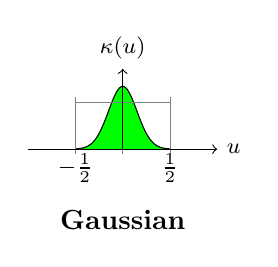
\begin{tikzpicture}[scale=.6,domain=-1:1]
\fill[color=green, samples=50] plot (\x,{1/(.3*sqrt(2*pi))*exp(-(\x*\x)/(2*.09))})--cycle;
\draw[color=black, samples=50] plot (\x,{1/(.3*sqrt(2*pi))*exp(-(\x*\x)/(2*.09))});
  \draw[very thin,color=gray] (-1,-0.1) grid (1,1.1);
  \draw[->] (-2,0) -- (2,0) node[right] {\footnotesize $u$};
  \draw[->] (0,0) -- (0,1.7) node[above] {\footnotesize $\kappa(u)$};
  \draw(1,-0.4) node {\footnotesize $\frac{1}{2}$};
  \draw(-1,-0.4) node {\footnotesize $-\frac{1}{2}$};
  \node at (0,-1.5) {\textbf{Gaussian}};
\end{tikzpicture}
\caption{Gaussian kernel}
\end{subfigure}
\hfill
\begin{subfigure}{0.32\textwidth}
\centering
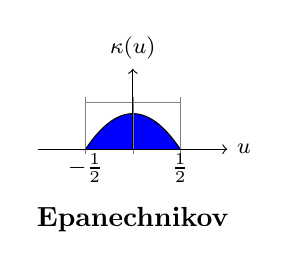
\begin{tikzpicture}[scale=.6,domain=-1:1]
\fill[color=blue, samples=50] plot (\x,{3/4*(1-\x*\x)})--cycle;
\draw[color=black, samples=50] plot (\x,{3/4*(1-\x*\x)});
  \draw[very thin,color=gray] (-1,-0.1) grid (1,1.1);
  \draw[->] (-2,0) -- (2,0) node[right] {\footnotesize $u$};
  \draw[->] (0,0) -- (0,1.7) node[above] {\footnotesize $\kappa(u)$};
  \draw(1,-0.4) node {\footnotesize $\frac{1}{2}$};
  \draw(-1,-0.4) node {\footnotesize $-\frac{1}{2}$};
  \node at (0,-1.5) {\textbf{Epanechnikov}};
\end{tikzpicture}
\caption{Epanechnikov kernel}
\end{subfigure}
\caption{Common kernel functions for Parzen window density estimation.}\label{f:kernels}
\end{figure}

\subsubsection*{Bandwidth selection}

The preceding discussion makes clear that the bandwidth \(h\) is the central hyperparameter of kernel density estimation. If \(h\) is chosen too large the estimator becomes biased; if \(h\) is chosen too small the estimator becomes unstable. In practice, \(h\) is tuned either by heuristic rules or by data-driven criteria.

A well-known ``rule of thumb'' (motivated by optimality calculations under Gaussian assumptions) takes the form
\[
h^* = 1.06\,\hat{\sigma}\,n^{-1/5},
\]
where \(\hat{\sigma}\) is the sample standard deviation (or an appropriate multivariate analogue). More generally, one can choose \(h\) by cross-validation. A common criterion maximizes the leave-one-out log-likelihood:
\begin{myequation}
h^* = \argmax{h}\ \frac{1}{n}\sum_{i=1}^{n} \log p_{-i}(\mathbf{x}_i),
\end{myequation}
where \(p_{-i}(\mathbf{x}_i)\) denotes the density estimate at \(\mathbf{x}_i\) computed using all samples except \(\mathbf{x}_i\). This criterion directly measures how well the estimated density predicts unseen data points.

\medskip

\subsubsection*{Classification via kernel density estimation}

Kernel density estimation becomes a classification method when it is applied class-wise. Suppose that for each class \(C_i\) we collect the subset of training points belonging to that class and build an estimate of \(p(\mathbf{x}\mid C_i)\):
\begin{myequation}
p(\mathbf{x}\mid C_i)=\frac{1}{n_i}\sum_{j:\,t_j=i}\kappa_h(\mathbf{x}-\mathbf{x}_j),
\end{myequation}
where \(n_i\) is the number of training samples in class \(C_i\). The class prior can be estimated empirically as \(p(C_i)=n_i/n\). Then Bayes’ rule yields a posterior proportional to \(p(\mathbf{x}\mid C_i)p(C_i)\), and a natural decision rule is
\begin{myequation}
\hat{C}=\argmax{i}\ p(\mathbf{x}\mid C_i)p(C_i).
\end{myequation}
This is a nonparametric analogue of generative classification: instead of assuming a parametric form for \(p(\mathbf{x}\mid C_i)\), we estimate it directly from data.

\medskip

\subsection*{\(k\)-Nearest Neighbors: fixed \(k\), variable volume}

\subsubsection*{The \(k\)-NN principle}

The \(k\)-nearest neighbors method starts from the same identity \(p(\mathbf{x})\approx k/(nV)\) but enforces locality in a different way. Instead of fixing the volume \(V\) and counting how many points fall inside, we fix the number of neighbors \(k\) and let the region expand until it contains exactly \(k\) samples. This adaptation is particularly appealing because it automatically adjusts to local data density: in dense regions the required neighborhood is small, while in sparse regions the neighborhood must expand.

Let \(r_k(\mathbf{x})\) denote the distance from \(\mathbf{x}\) to its \(k\)-th nearest neighbor. If we use as region \(\mathcal{R}(\mathbf{x})\) a \(d\)-dimensional ball of radius \(r_k(\mathbf{x})\), its volume is \(V=c_d\,r_k(\mathbf{x})^d\), where \(c_d\) is the volume of the unit \(d\)-dimensional ball. The resulting density estimate becomes
\begin{myequation}
p(\mathbf{x})\approx \frac{k}{n\cdot c_d\cdot r_k(\mathbf{x})^d}.
\end{myequation}
This expression makes explicit how density is inversely related to the radius needed to capture \(k\) points: where the data are dense, \(r_k(\mathbf{x})\) is small and the estimated density is high.

\medskip

\subsubsection*{\(k\)-NN classification}

For classification, the most common \(k\)-NN rule does not even require an explicit density estimate. Given a query \(\mathbf{x}\), we find its \(k\) nearest training points and count how many belong to each class. Let \(k_i\) be the number of these neighbors in class \(C_i\). One can motivate the standard majority vote rule through a probabilistic argument.

If we approximate the class-conditional density within the local region \(\mathcal{R}(\mathbf{x})\) by local counts, we obtain
\begin{myalign}
p(\mathbf{x}\mid C_i) &= \frac{k_i}{n_i V},\\
p(\mathbf{x}) &= \frac{k}{nV}.
\end{myalign}
Substituting into Bayes’ rule and using \(p(C_i)=n_i/n\), we get
\begin{myalign}
p(C_i\mid \mathbf{x})
&=\frac{p(\mathbf{x}\mid C_i)p(C_i)}{p(\mathbf{x})}
=\frac{\frac{k_i}{n_i V}\cdot \frac{n_i}{n}}{\frac{k}{nV}}
=\frac{k_i}{k}.
\end{myalign}
Thus the posterior probability is approximated simply by the fraction of neighbors in each class. The resulting decision rule is therefore
\begin{myequation}
\hat{C}=\argmax{i}\ k_i,
\end{myequation}
which is exactly majority voting among the \(k\) nearest neighbors. The remarkable simplicity of this rule is one reason \(k\)-NN is frequently used as a baseline method in classification.

\medskip

\subsubsection*{\(k\)-NN examples and decision boundaries}

The value of \(k\) controls the smoothness of the resulting decision boundary. Small \(k\) yields highly flexible boundaries that can track individual training samples, while large \(k\) produces smoother boundaries that may underfit. The following figures illustrate this behavior for a two-dimensional dataset:

\begin{figure}[h]
\centerline{
\includegraphics[width=0.25\textwidth]{Figure2-28a.pdf}}
\end{figure}

\begin{figure}[h]
\centerline{
\includegraphics[width=0.25\textwidth]{Figure2-28b.pdf}}
\end{figure}

\begin{figure}[h]
\centerline{
\includegraphics[width=0.25\textwidth]{Figure2-28c.pdf}}
\end{figure}

\subsubsection*{Theoretical properties and practical considerations}

From a theoretical standpoint, \(k\)-NN has appealing asymptotic properties. With appropriate choices of \(k\) as a function of \(n\), the method is consistent and approaches the Bayes optimal error rate as \(n\to\infty\). At the same time, its finite-sample behavior depends strongly on design choices.

The most important choice is \(k\). When \(k=1\), the classifier is extremely local and can overfit: every training point becomes a ``prototype'' with its own small region of influence. As \(k\) increases, predictions average over more samples and become more stable, but the boundary may become too smooth. In practice, \(k\) is chosen by cross-validation or by simple heuristics such as \(k\approx \sqrt{n}\), keeping in mind that the optimal value depends on noise level, class overlap, and dimension.

Another critical aspect is the \emph{distance metric}. Nearest-neighbor methods rely entirely on the notion of distance, so feature scaling and metric selection (Euclidean, Manhattan, Mahalanobis, cosine distance, etc.) can dramatically affect performance. In high-dimensional spaces, distances tend to concentrate, weakening the notion of ``nearest'' and worsening performance---one of the many manifestations of the curse of dimensionality.

Finally, there are computational considerations. \(k\)-NN is often described as a \emph{lazy} learning method: it performs minimal computation during training (essentially storing the dataset) and defers most effort to prediction time, where a nearest-neighbor search is required. A naive search costs \(O(n)\) per query. Acceleration structures such as KD-trees or ball trees can reduce the typical cost for low to moderate dimensions, although the benefits diminish as dimensionality increases.

\medskip

\subsubsection*{\(k\)-NN vs.\ kernel density estimation}

Kernel density estimation and \(k\)-NN can be viewed as two sides of the same local counting principle. KDE fixes the region size and lets the number of points vary; \(k\)-NN fixes the number of points and lets the region size vary. Each choice has consequences. KDE can be convenient when a natural scale \(h\) is known or can be tuned, and it yields smooth density estimates by construction. \(k\)-NN automatically adapts neighborhood size to local sample density, which can be advantageous in heterogeneous datasets, but its prediction rule can be less smooth for small \(k\).

\medskip

\subsection*{Summary: nonparametric density methods}

Kernel density estimation and \(k\)-nearest neighbors are canonical examples of nonparametric methods for density estimation and classification. Both implement a locality principle through neighborhoods around query points, and both become more expressive as the dataset grows. Their strengths lie in flexibility and, under suitable conditions, consistency. Their limitations lie in computational cost and in the curse of dimensionality, which can make naive locality assumptions ineffective in high-dimensional spaces. Despite these challenges, nonparametric methods remain valuable as practical baselines, as conceptual tools for understanding density-based learning, and as building blocks for more sophisticated modern algorithms.


%\end{document}